\documentclass[12pt]{article}
\usepackage[utf8]{inputenc}
\usepackage[czech]{babel}
\usepackage{enumitem}
\usepackage{caption}
\usepackage{url}
\usepackage{graphicx}
\usepackage{footnote}
\makesavenoteenv{tabular}

\begin{document}

\begin{center}
\bf Semestrální projekt MI-PAP 2015/2016:\\[5mm]
    Modelování částic\\[5mm]
       Miroslav Brabenec\\
       Jan Nováček\\[2mm]
magisterské studium, FIT ČVUT, Thákurova 9, 160 00 Praha 6\\[2mm]
\today
\end{center}
%
%
%
% Co má být ve zprávě: https://edux.fit.cvut.cz/courses/MI-PAP/labs/technicka_zprava
%
%
\section{Definice problému, popis sekvenčního algoritmu a jeho implementace}

\subsection{Definice problému}
Implementujte tento algoritmus (viz \url{http://www.browndeertechnology.com/docs/BDT_OpenCL_Tutorial_NBody-rev3.html#algorithm}) a upravte ho takto:

\begin{enumerate}
\item	částice při nárazu provedou pružný odraz a
\item	každá částice má svůj náboj
\end{enumerate}

Úkol: doplňte o možnost vizualizace (alespoň exportem dat v daných časových okamžicích ve formátu vhodném pro vizualizaci v nástroji třetích stran např. ) 

\subsection{Popis sekvenčního algoritmu}
Simulátor načte nastavení simulace a počáteční umístění částic ze vstupního souboru, z toho nainicializuje hodnoty a spustí simulaci.

Simulace běží, dokud ...

\subsection{Sekvenční implementace}

Bylo implementováno několik sekvenčních variant, lišících se v míře ruční vektorizace struktur použitých v algoritmu.

První varianta (V1) používá pouze automatickou vektorizaci (přepínač -O3), nepoužívala žádné SSE instrukce ani ručně vytvořené vektory.

V druhě variantě (V2) je automatická vektorizace (-O3) a SSE instrukce pro výpočet ${\frac{1}{\sqrt{x}}}$.

V třetí variantě (V3) je automatická vektorizace (-O3), SSE datové typy~\_\_m128 a SSE in\-struk\-ce pro výpočet ${\frac{1}{\sqrt{x}}}$.

Porovnání rychlostí jednotlivých sekvenčích implementací je v tabulce níže.

\begin{center}
\begin{tabular}{c | c | c | c | c}
\textbf{Počet částic} & \textbf{Počet kroků sim.}  & \textbf{V1} & \textbf{V2} & \textbf{V3} \\ \hline \hline
1024 & 50 000 & 760.19s & 574.16s & 101.88s \\ \hline
512 & 400 000 & 1526.06s & 1198.62s & 206.92s \\ \hline
4096 & 5 000 & 1215.77s & 887.54s & 160.28s \\ \hline
\end{tabular}
\captionof{table}{Časy sekvenčních implementací}
\end{center}

\section{Popis paralelního algoritmu a jeho implementace v OpenMP}
%Popis případných úprav algoritmu a jeho implementace, včetně volby datových struktur


% Zda byla využita vektorizace (popř. proč jí nemožno využít)
\subsection{Vektorizace}

V prog\-ramu byla nej\-prve pou\-žita au\-toma\-tická vekto\-ri\-za\-ce (-O3).
Její výsledek měl na rychlost výpočtu minimální vliv. Za nejkritičtější část kódu byla vyhodnocena část, kde se počítá ${\frac{1}{\sqrt{x}}}$.
Pro tento úsek kódu lze využít speciální vektorové instrukce. Použitím této instrukce došlo ke znatelnému zrychlení výpočtu.
V další fázi byl kód upraven, tak aby bylo možné využít vektorové instrukce které dokáží počítat paralelně několik hodnot ${\frac{1}{\sqrt{x}}}$.
Zde byly částice rozděleny do chunků po 4 a v každém kroku se počítá ovlivnění částice chunkem částic.
Díky tomu je možné počítat 4 inverzní odmocniny naráz a dochází k rapidnímu zrychlení. 

% Popis optimalizací pro dosažení lineárního zrychlení
\subsection{Optimalizace}

Pro vektorizaci byly využity technologie obsažené v SSE2. Dalšího zrychlení by bylo možno dosáhnout při použití novějších vektorových instrukcí.
Ty by měly umožňovat tvorbu chunků o velikosti 8, případně 16.
Dále by také bylo možno upravit kód, tak aby docházelo k počítání vzdálenosti mezi částicemi pouze jednou.
Momentálně se počítá vzdálenost mezi částicemi A a B dvakrát, jednou z pohledu částice A a jednou z pohledu částice B.

\subsection{Vstupní data}

Pro měření jsme vytvořili 3 vzorky dat. Vzorky dat se lišily v počtu částic a počtu kroků simulace.
Všechny vzorky byly srovnatelné co se týče výpočetní náročnosti. Výpočetní náročnost lze spočítat jako ${N = P^2 \times S}$, kde P = počet částic a S = počet kroků.
Efektivita paralelního výpočtu se zlepšuje s rostoucím počtem částic.

\begin{center}
\begin{tabular}{c | c | c }
\textbf{Počet částic} & \textbf{Počet kroků sim.}  & \textbf{Výpočetní náročnost}\footnote{Spočítáno podle vzorce ${\frac{P^2 \times S}{10^9}}$, kde P = počet částic a S = počet kroků} \\ \hline \hline
1024 & 50 000 & 52,428 \\ \hline
512 & 400 000 & 104,857 \\ \hline
4096 & 5 000 & 83,804 \\ \hline
\end{tabular}
\captionof{table}{Časy sekvenčních implementací}
\end{center}

% Tabulkově a případně graficky zpracované naměřené hodnoty časové složitosti měřených instancí běhu (optimalizované implementace) programu s popisem instancí dat
\section{Naměřené výsledky a vyhod\-noce\-ní pro O\-pen\-MP}

\subsection{Měření pro variantu 2}
První měření bylo prováděno na vstupních datech velikosti XX částic a YY kroků simulace.

\begin{center}
\begin{tabular}{ c | c }
\textbf{Počet vláken} & \textbf{Naměřený čas} \\ \hline \hline 
1 & 574.160156s \\ \hline
2 & 342.273438s \\ \hline
4 & 182.601562s \\ \hline
8 & 128.050781s \\ \hline
16 & 94.910156s \\ \hline
24 & 92.789062s \\ \hline
\end{tabular}
\captionof{table}{Časy 1. měření}
\end{center}

\begin{figure}[h]
  \begin{center}
     \includegraphics[width=12cm]{images/sse1.png}
    \caption{Měření 1. instance} 
  \end{center}
\end{figure}

Při prvním měření ...



\begin{center}
\begin{tabular}{ c | c }
\textbf{Počet vláken} & \textbf{Naměřený čas} \\ \hline \hline 
1 & 1198.617188s \\ \hline
2 & 758.753906s \\ \hline
4 & 480.691406s \\ \hline
8 & 439.945312s \\ \hline
16 & 426.421875s \\ \hline
24 & 446.625000s \\ \hline
\end{tabular}
\captionof{table}{Časy 2. měření}
\end{center}

\begin{figure}[h]
  \begin{center}
    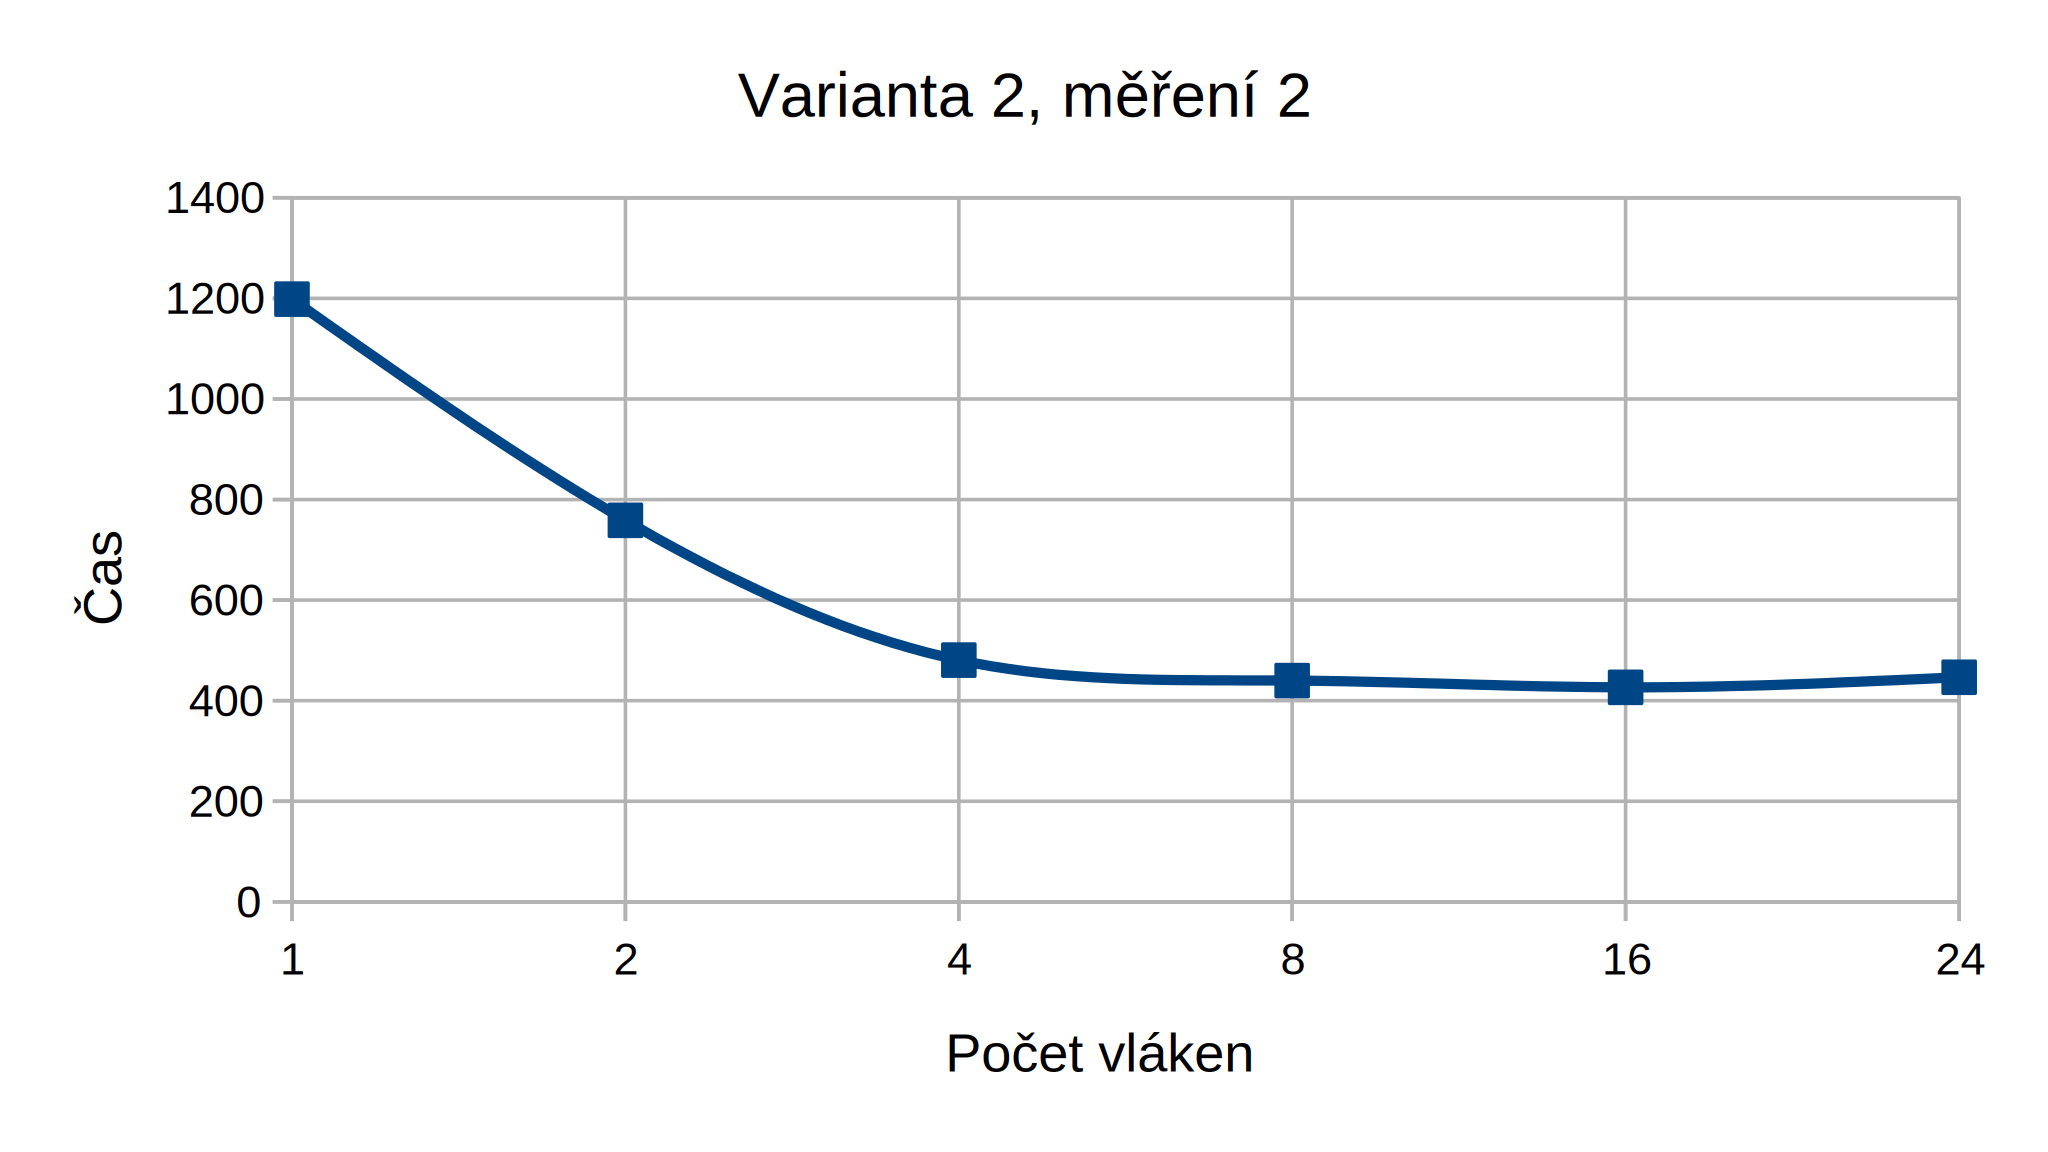
\includegraphics[width=12cm]{images/sse2.png}
    \caption{Měření 2. instance} 
  \end{center}
\end{figure}



\begin{center}
\begin{tabular}{ c | c }
\textbf{Počet vláken} & \textbf{Naměřený čas} \\ \hline \hline 
1 & 887.542969s \\ \hline
2 & 452.800781s \\ \hline
4 & 225.554688s \\ \hline
8 & 117.988281s \\ \hline
16 & 99.117188s \\ \hline
24 & 67.757812s \\ \hline
\end{tabular}
\captionof{table}{Časy 3. měření}
\end{center}

\begin{figure}[h]
  \begin{center}
     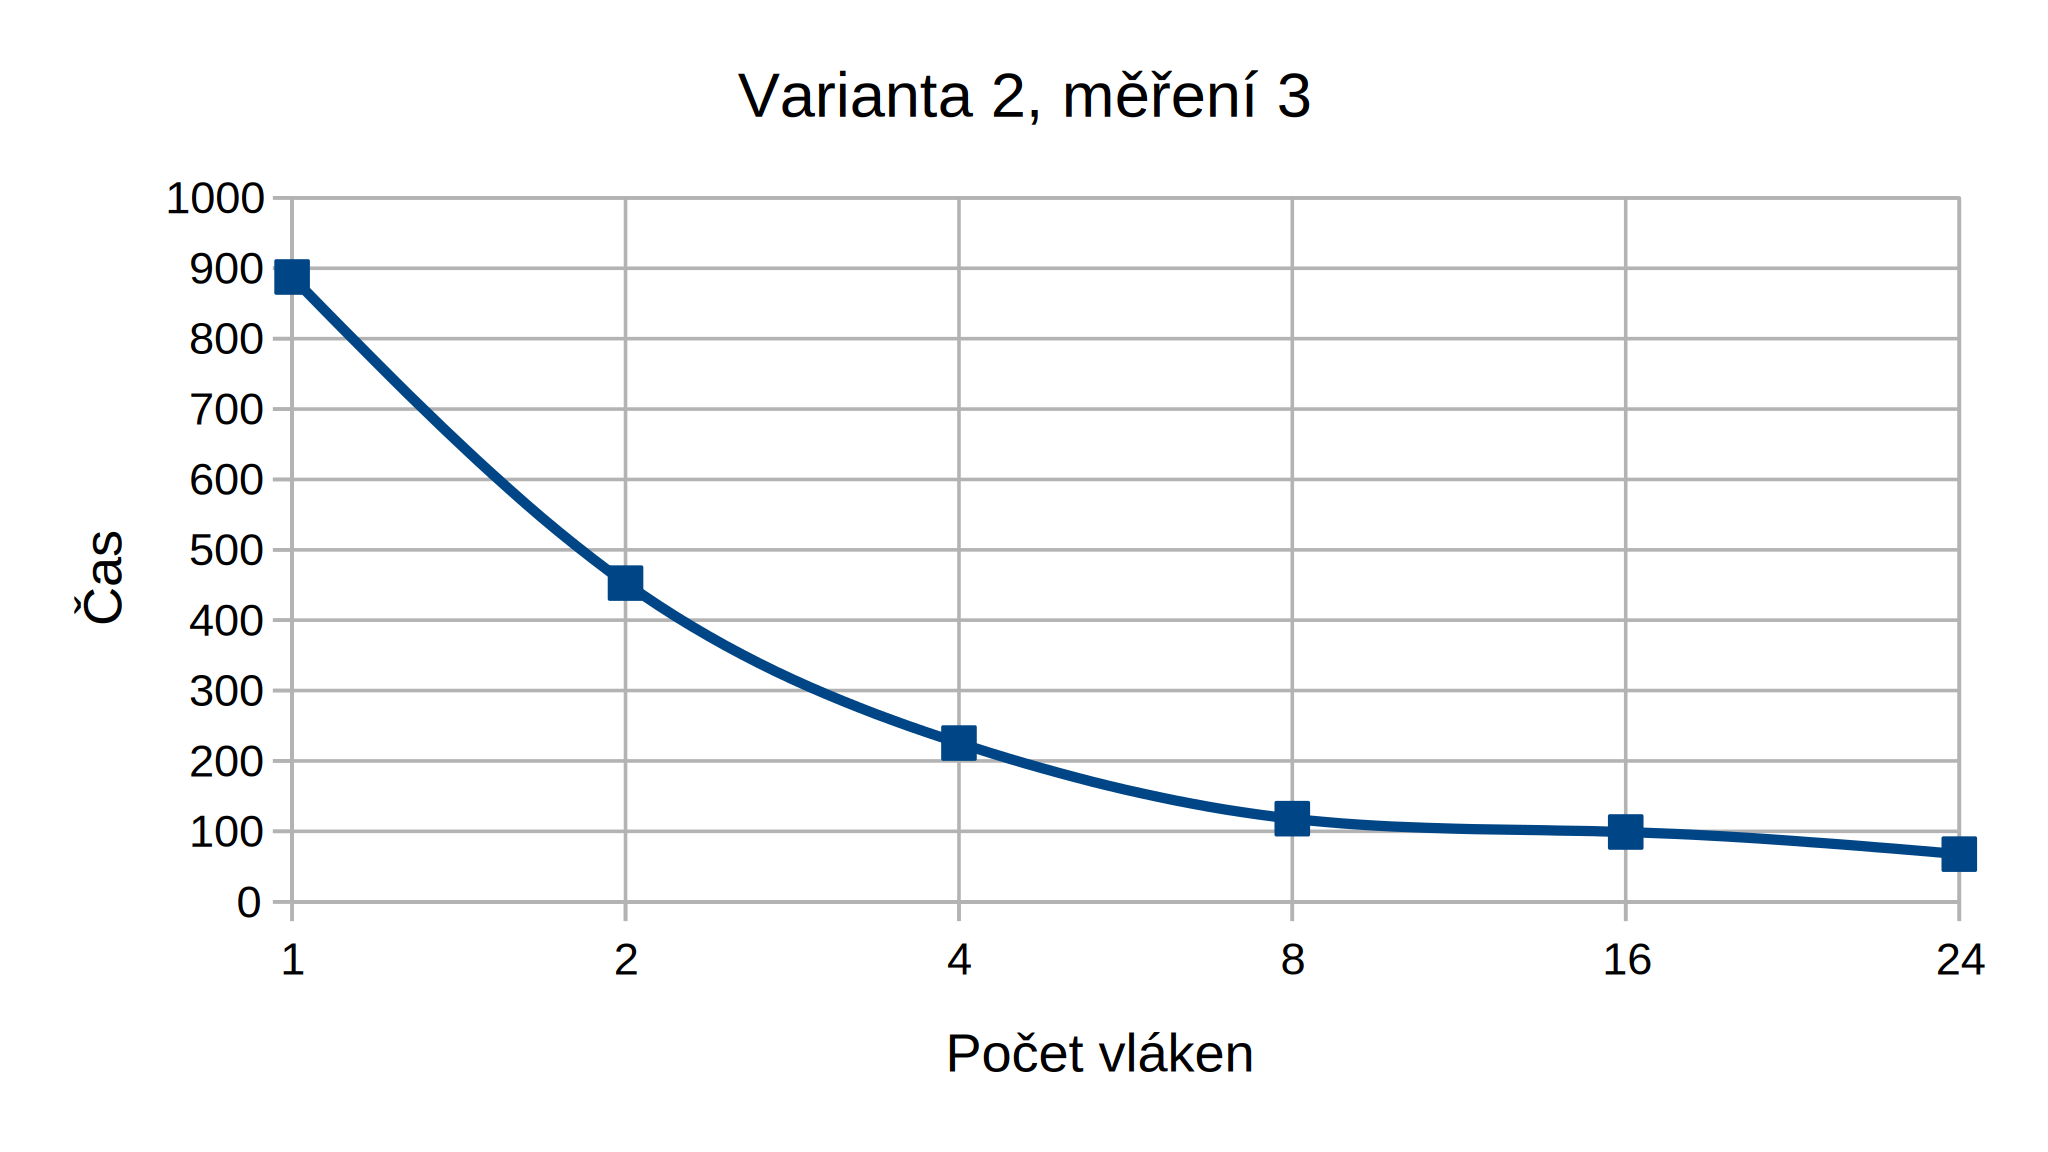
\includegraphics[width=12cm]{images/sse3.png}
    \caption{Měření 3. instance} 
  \end{center}
\end{figure}



\subsection{Měření pro variantu 3}
První měření bylo prováděno na vstupních datech velikosti XX částic a YY kroků simulace.

\begin{center}
\begin{tabular}{ c | c }
\textbf{Počet vláken} & \textbf{Naměřený čas} \\ \hline \hline 
1 & 101.878906s \\ \hline
2 & 107.039062s \\ \hline
4 & 69.917969s \\ \hline
8 & 63.246094s \\ \hline
12 & 69.171875s \\ \hline
24 & 44.578125s \\ \hline
\end{tabular}
\captionof{table}{Časy 1. měření}
\end{center}

\begin{figure}[h]
  \begin{center}
     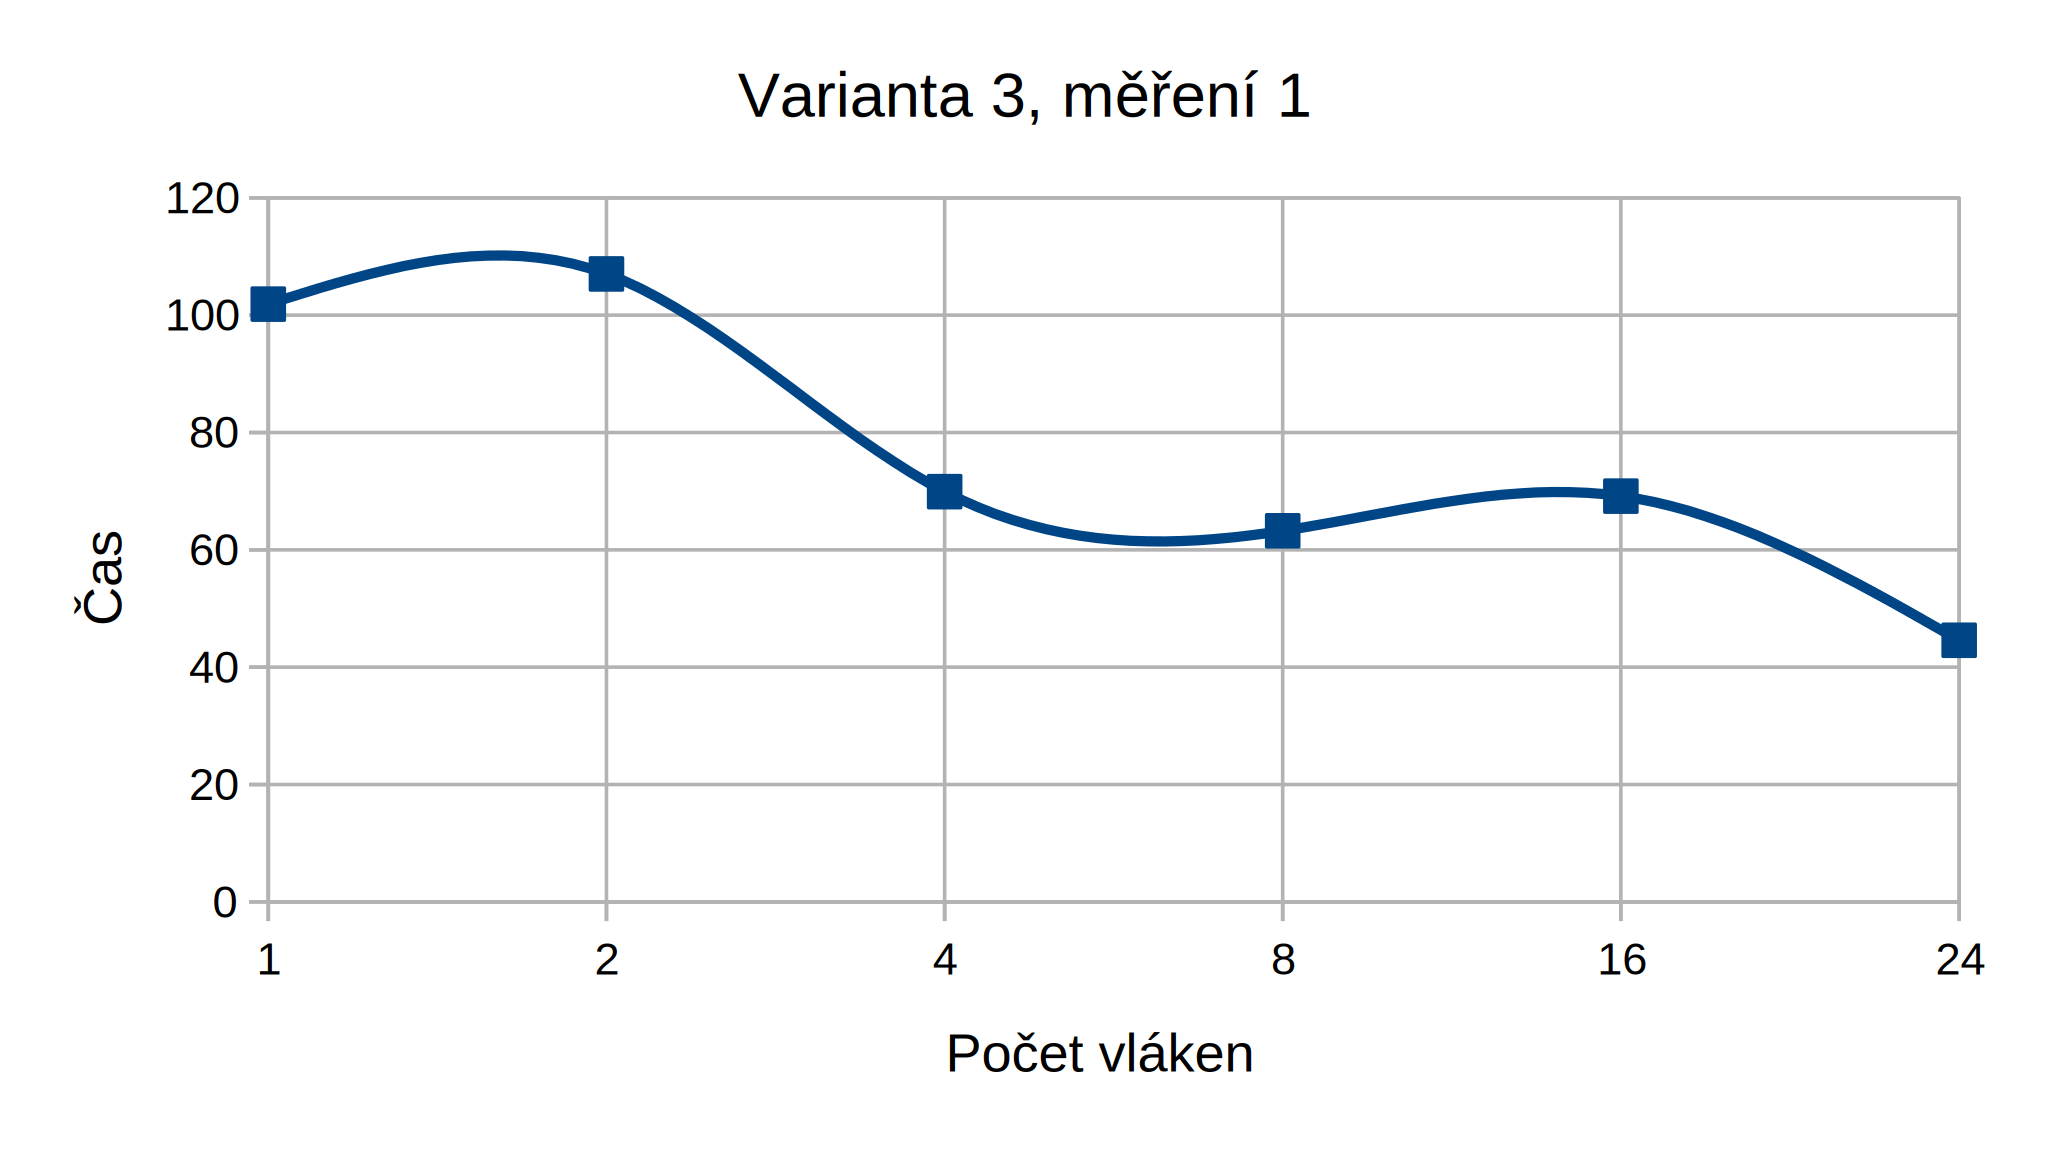
\includegraphics[width=12cm]{images/ssef1.png}
    \caption{Měření 1. instance} 
  \end{center}
\end{figure}

Při prvním měření ...



\begin{center}
\begin{tabular}{ c | c }
\textbf{Počet vláken} & \textbf{Naměřený čas} \\ \hline \hline 
1 & 206.921875s \\ \hline
2 & 214.226562s \\ \hline
4 & 201.382812s \\ \hline
8 & 234.585938s \\ \hline
16 & 227.109375s \\ \hline
24 & 191.773438s \\ \hline
\end{tabular}
\captionof{table}{Časy 2. měření}
\end{center}

\begin{figure}[t]
  \begin{center}
      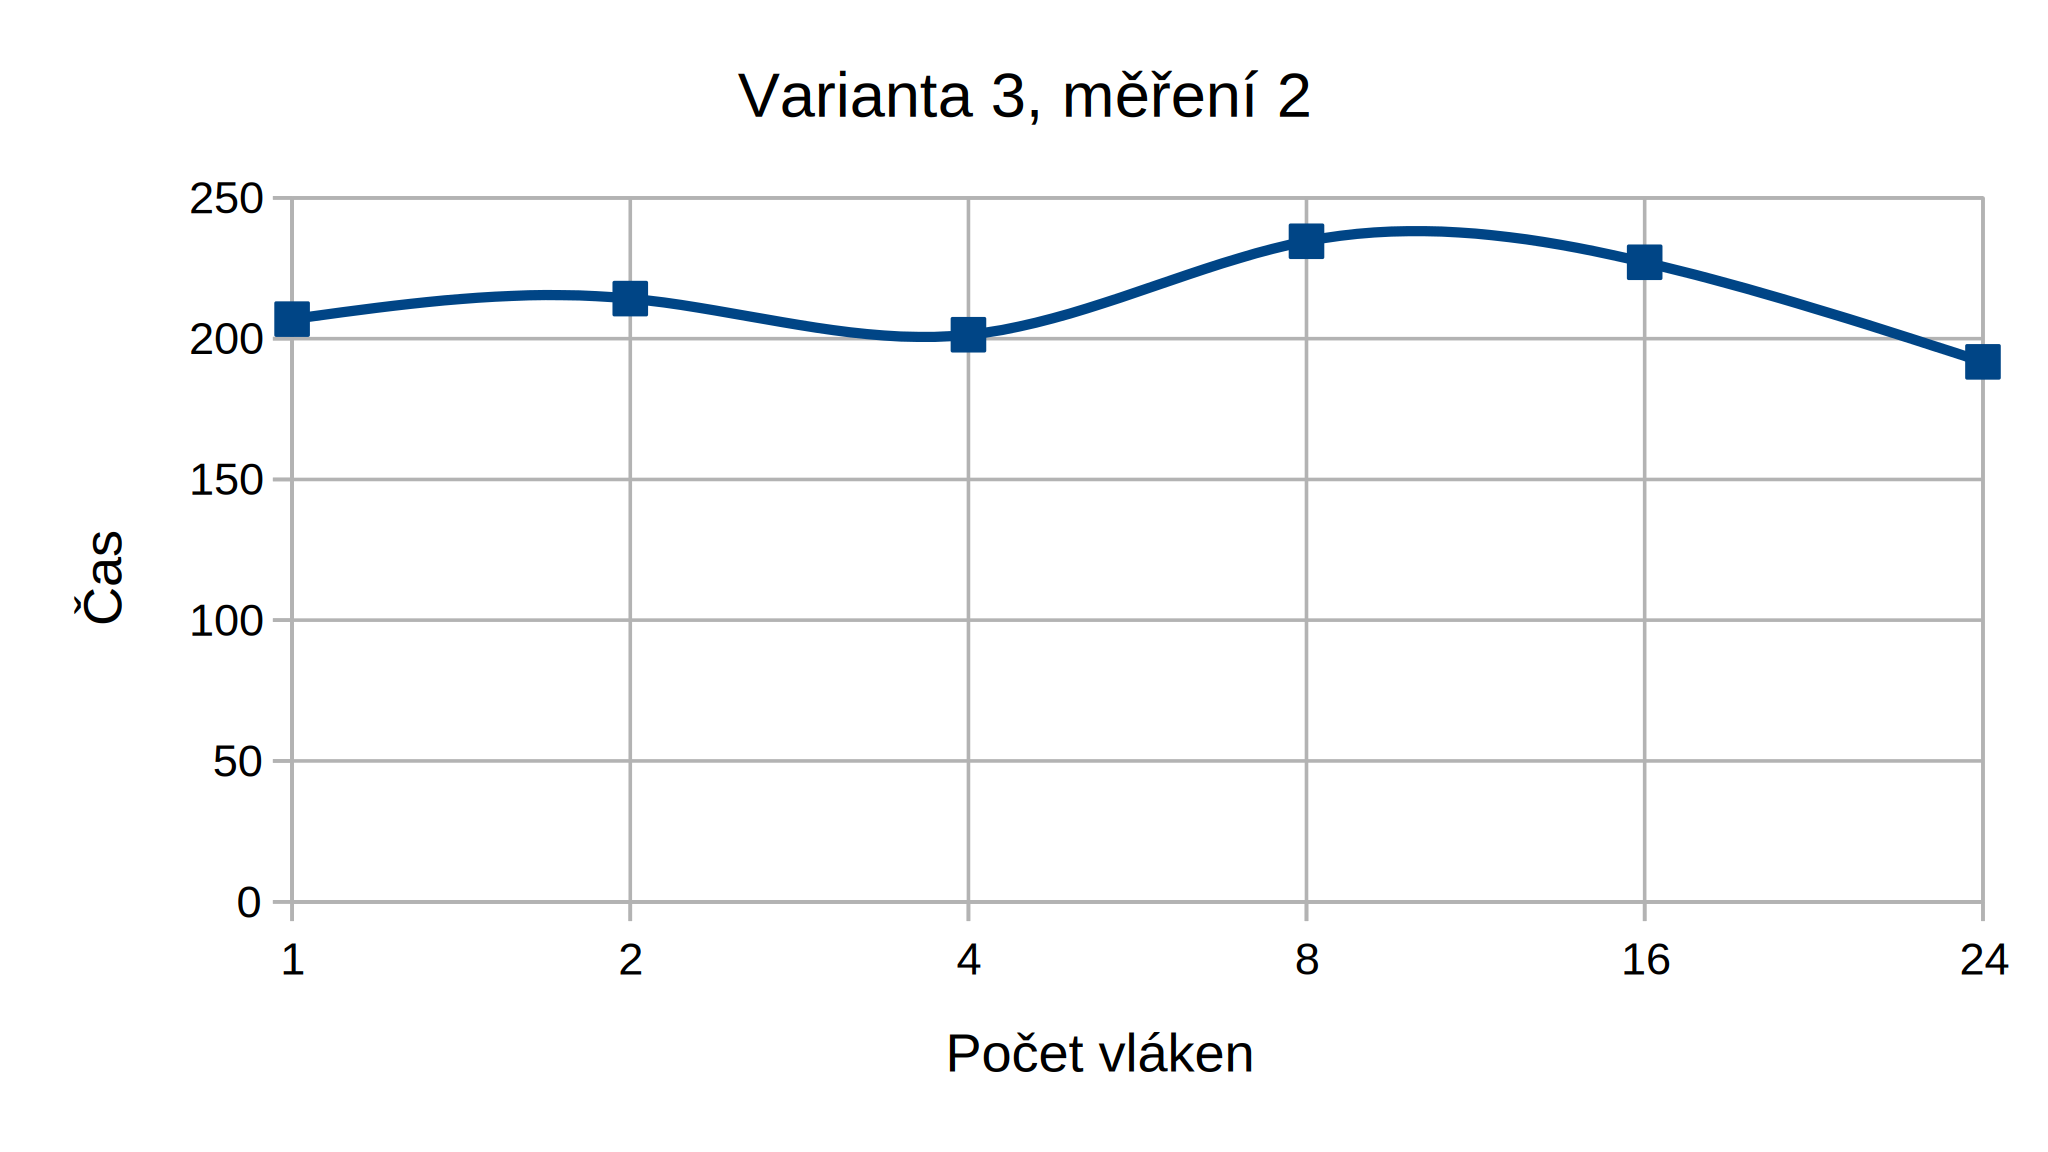
\includegraphics[width=12cm]{images/ssef2.png}
    \caption{Měření 2. instance} 
  \end{center}
\end{figure}




\begin{center}
\begin{tabular}{ c | c }
\textbf{Počet vláken} & \textbf{Naměřený čas} \\ \hline \hline 
1 & 160.281250s \\ \hline
2 & 97.597656s \\ \hline
4 & 50.394531s \\ \hline
8 & 41.648438s \\ \hline
16 & 26.859375s \\ \hline
24 & 20.953125s \\ \hline
\end{tabular}
\captionof{table}{Časy 3. měření}
\end{center}

\begin{figure}[t]
  \begin{center}
      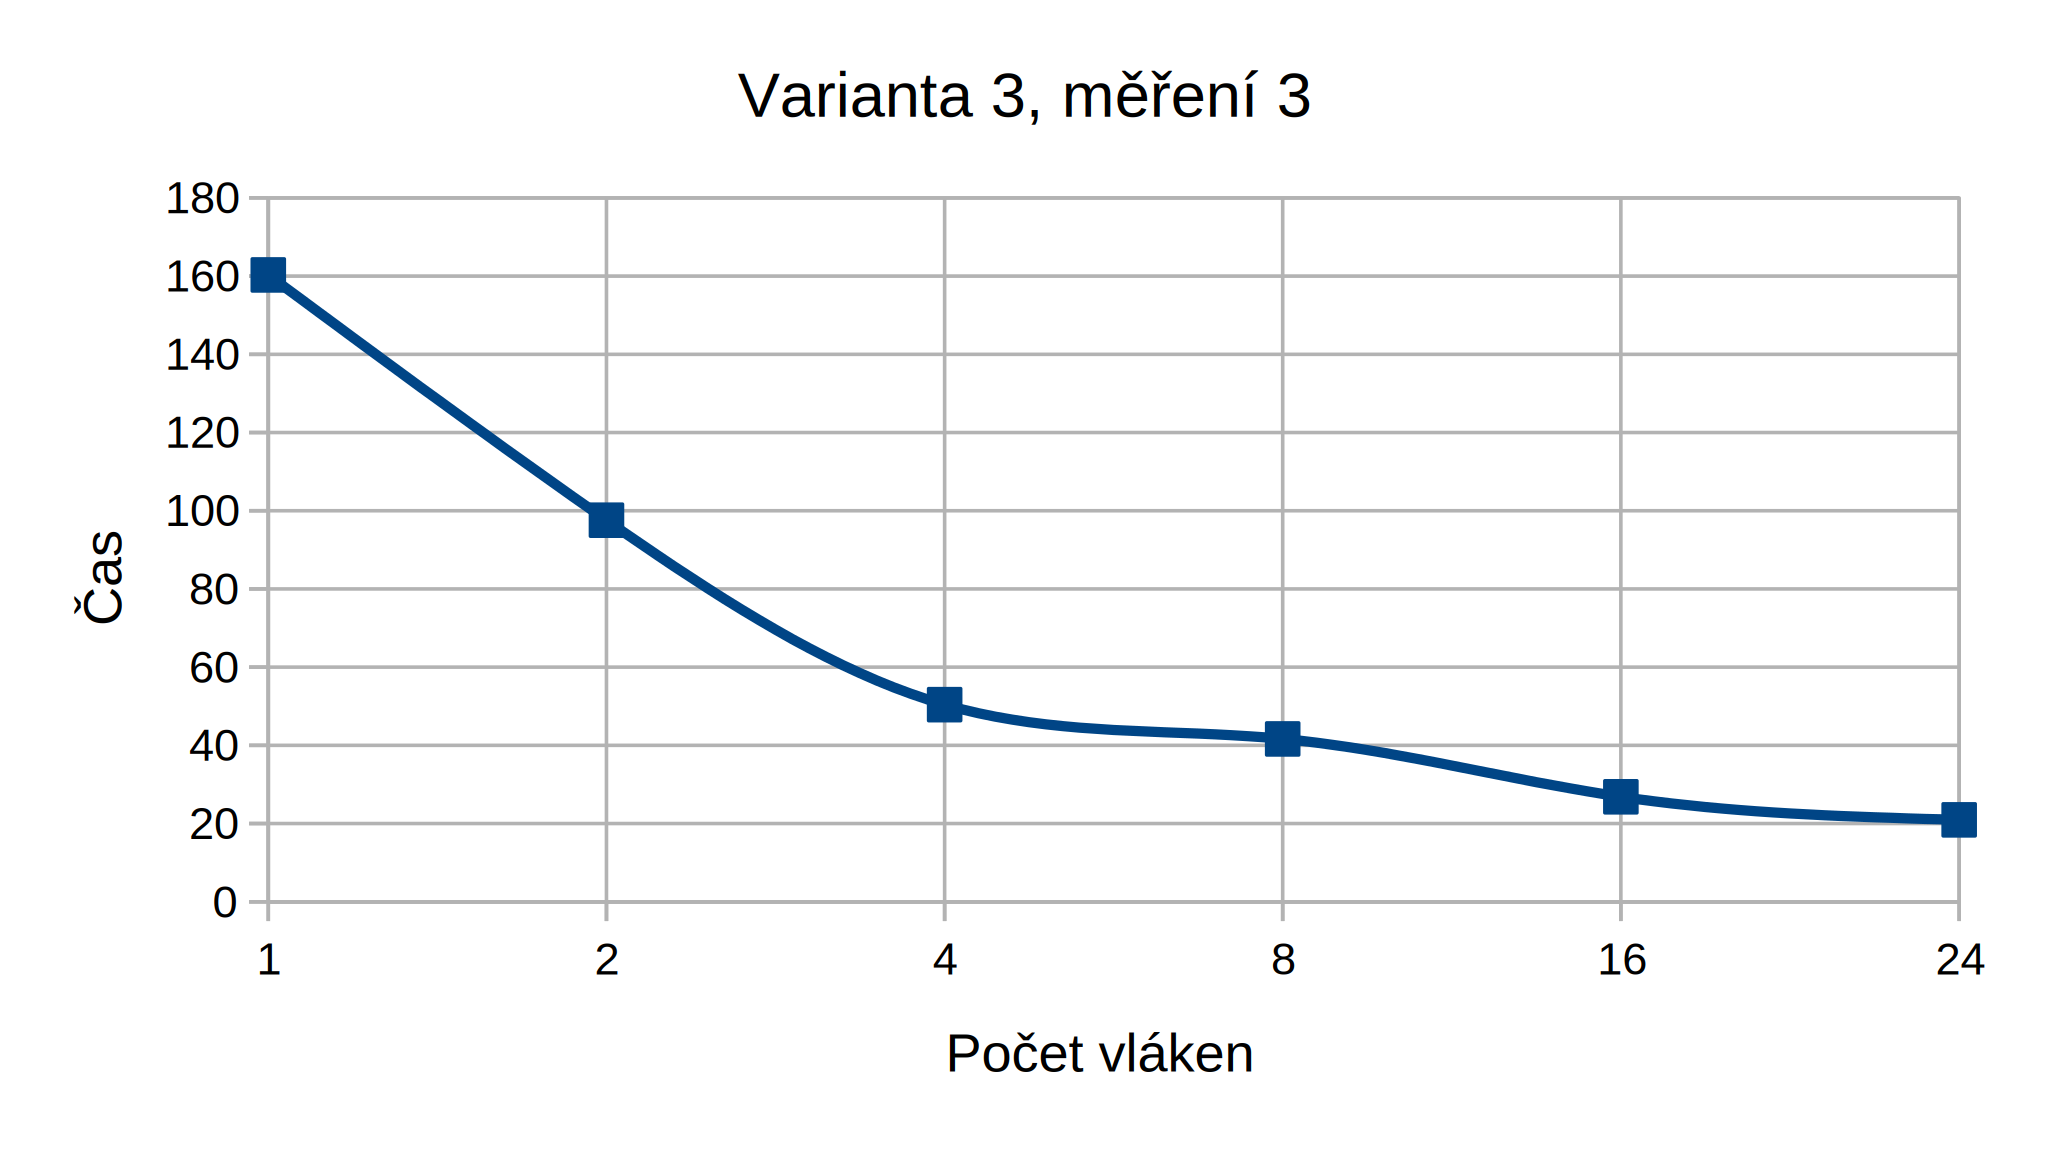
\includegraphics[width=12cm]{images/ssef3.png}	
    \caption{Měření 3. instance} 
  \end{center}
\end{figure}

% Analýza a hodnocení vlastností dané implementace programu.
\subsection{Porovnání jednotlivých impelentací}

\begin{figure}[h]
  \begin{center}
      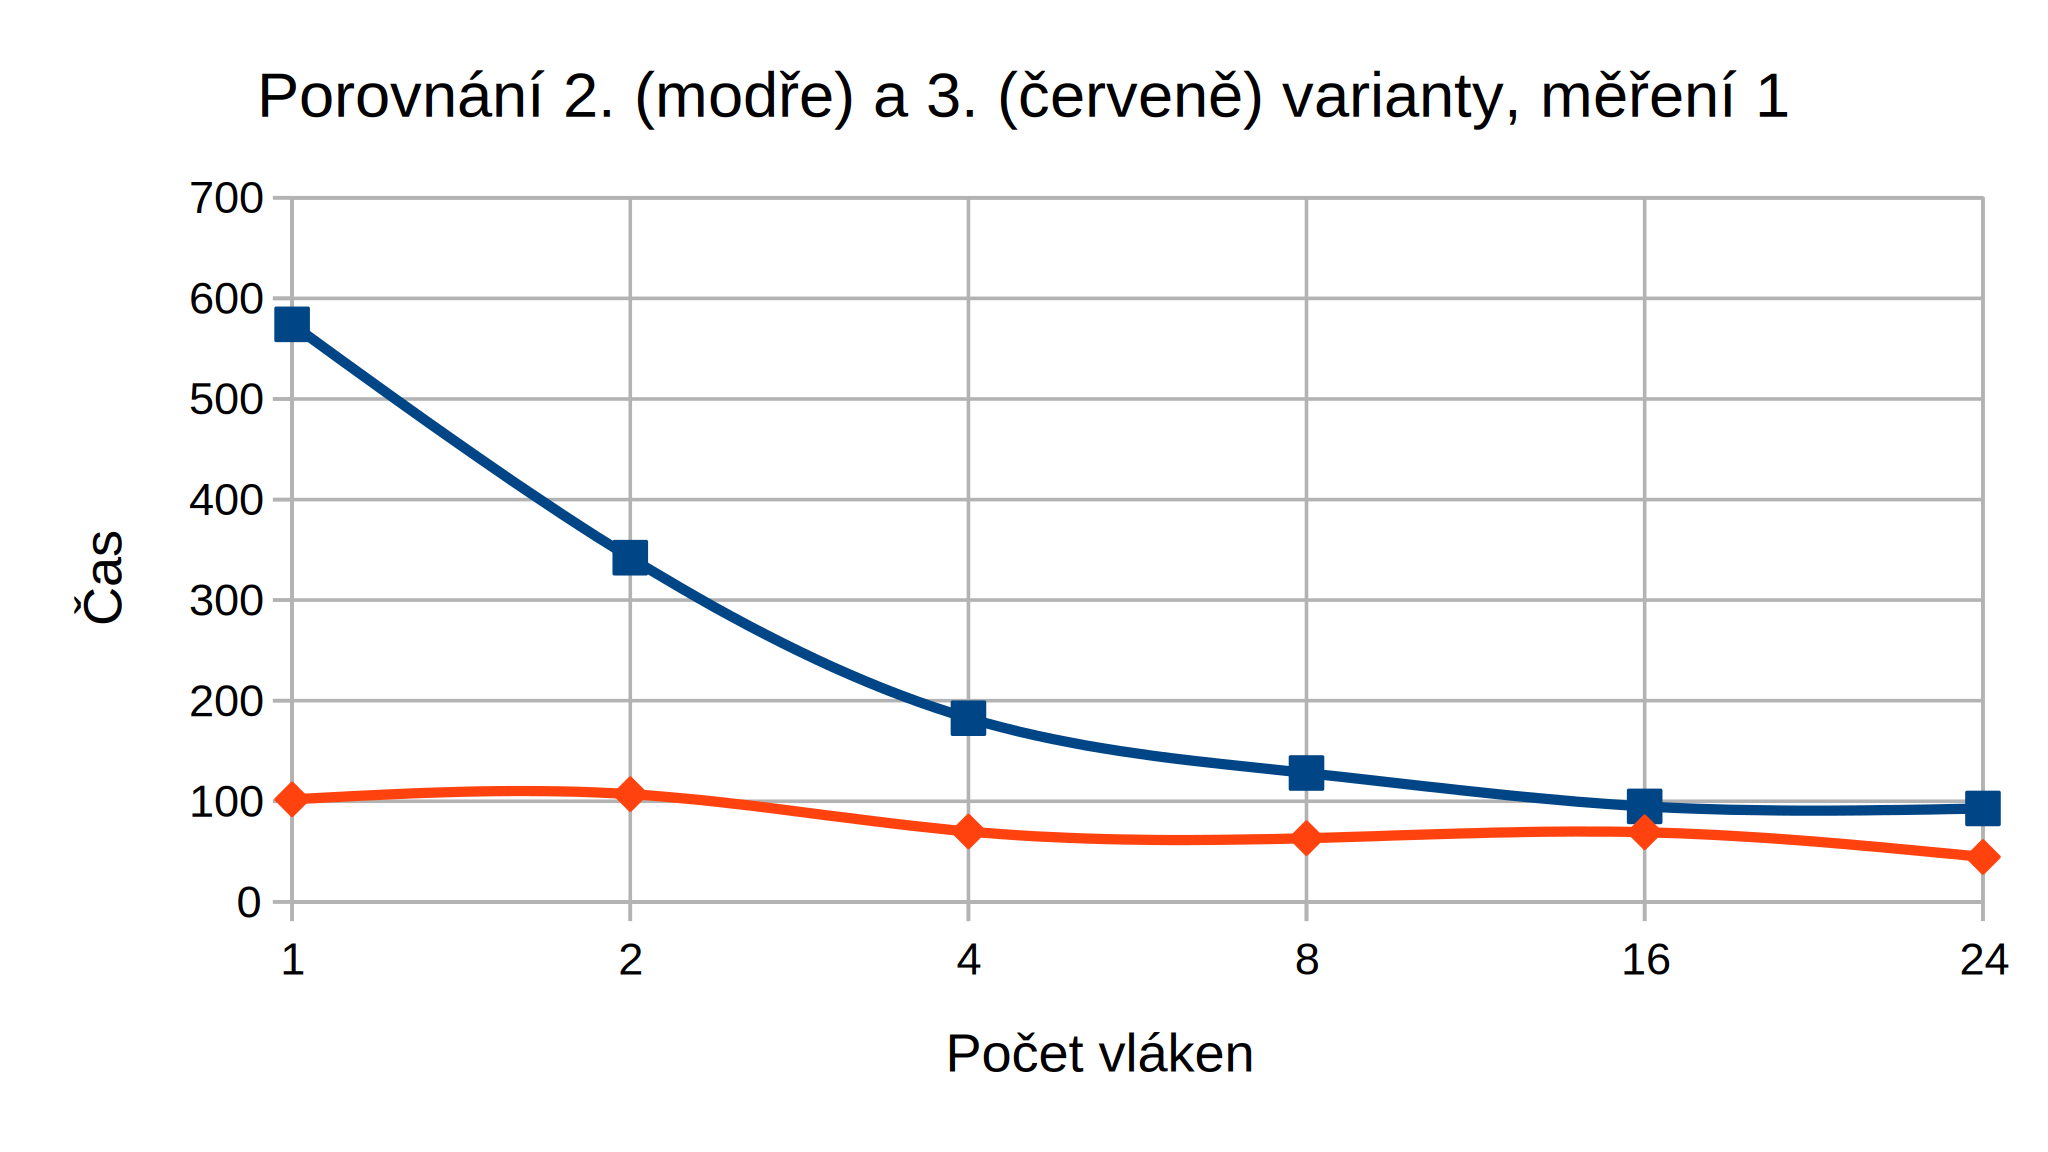
\includegraphics[width=12cm]{images/vs1.png}	
    \caption{Porovnání implementací, měření 1} 
  \end{center}
\end{figure}

\begin{figure}[h]
  \begin{center}
      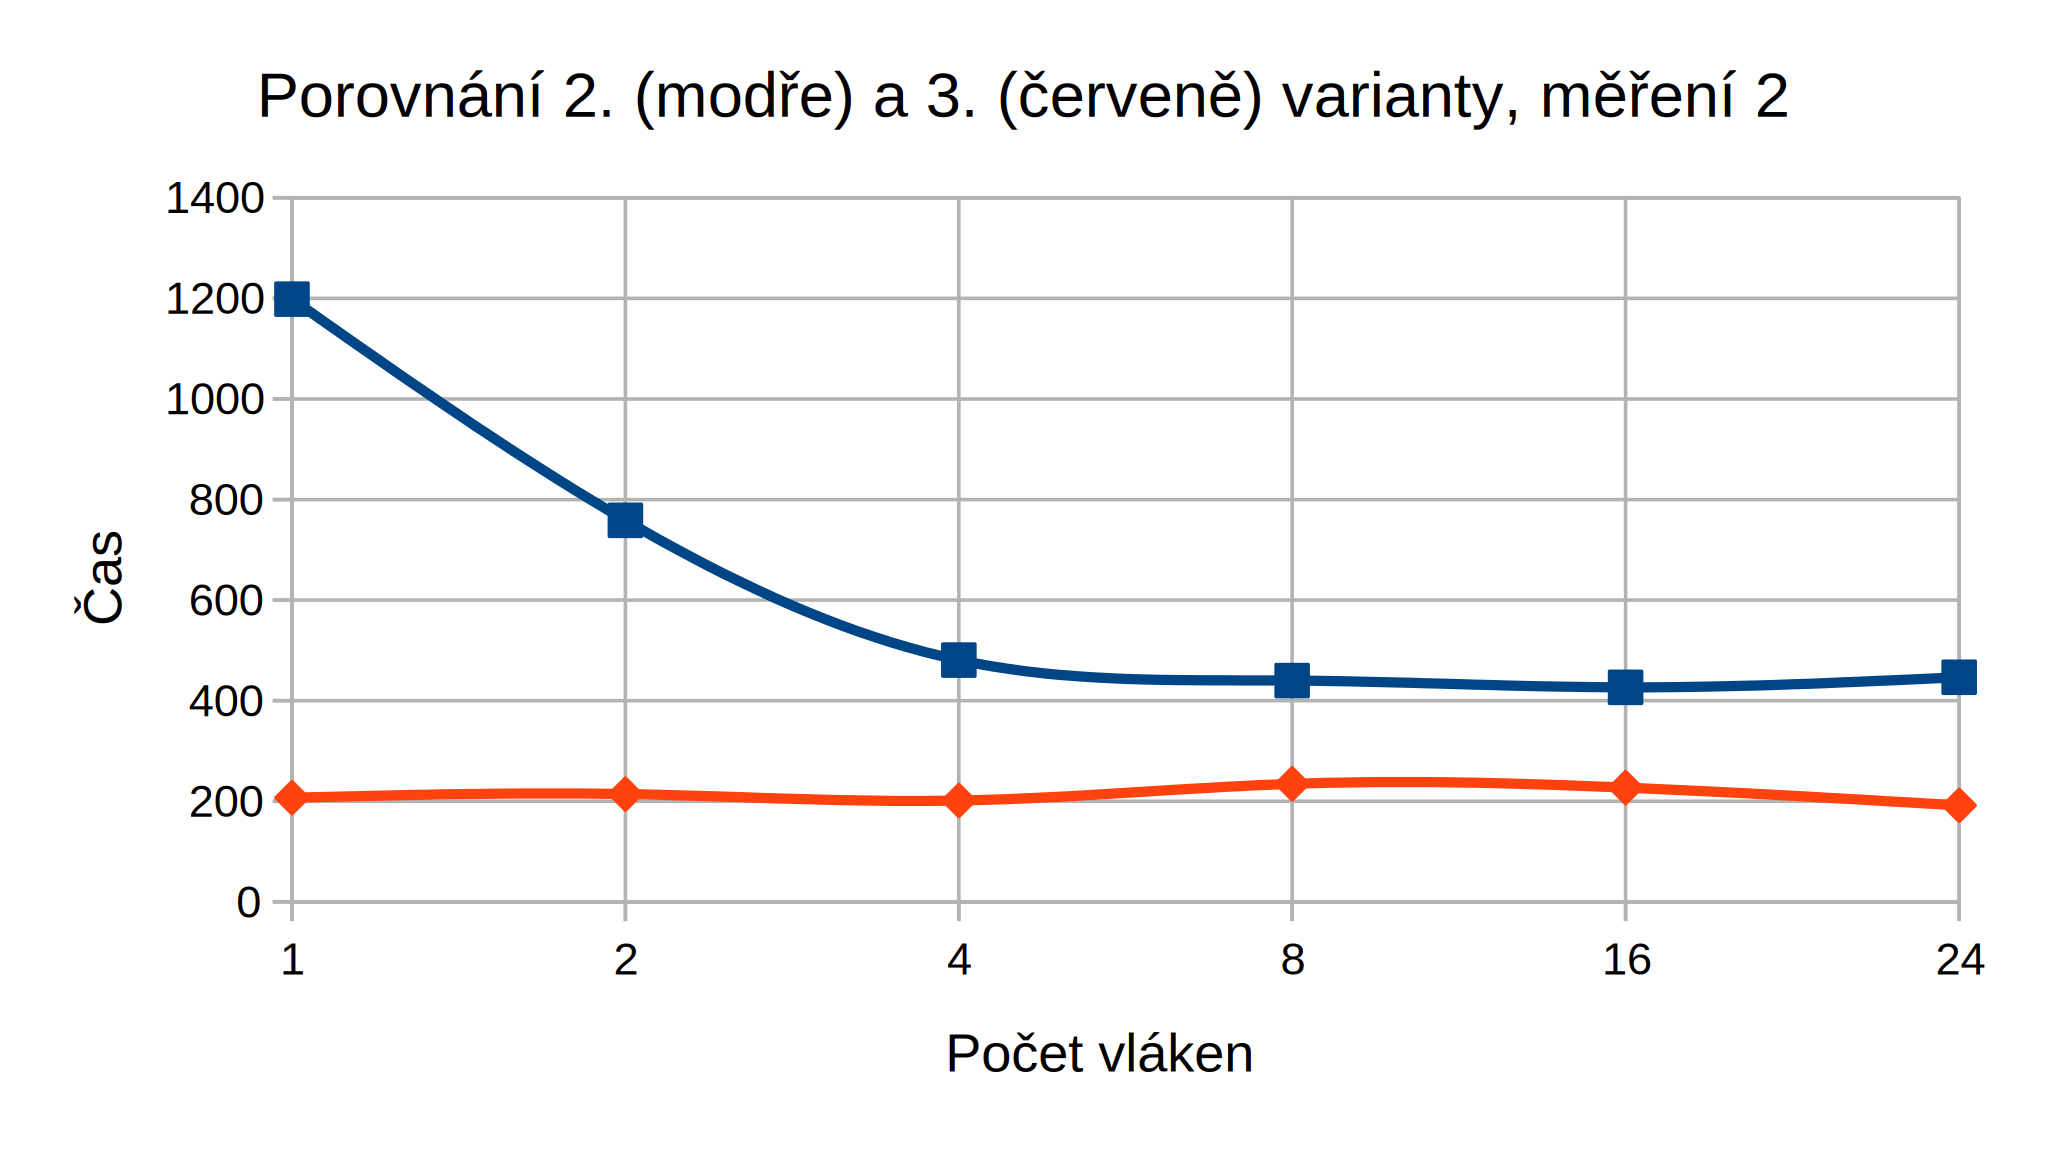
\includegraphics[width=12cm]{images/vs2.png}	
    \caption{Porovnání implementací, měření 2}
  \end{center}
\end{figure}

\begin{figure}[h]
  \begin{center}
      \includegraphics[width=12cm]{images/vs3.png}	
    \caption{Porovnání implementací, měření 3}
  \end{center}
\end{figure}


\end{document}
